\section{Algoritmo de Línea de Base}
Línea base es un proceso para estudiar la red a intervalos regulares para asegurarse de que la red está trabajando dentro de los parámetros normales. Permite obtener información valiosa como:

\begin{itemize}
	\item Salud de hardware y software.
	\item Uso de recursos de red.
	\item Umbrales de alarma.
	\item Problemas futuros en la red.
\end{itemize}

El proceso de línea base parte de un acuerdo de nivel de servicio (SLA) establecido entre el proveedor de servicio y sus clientes sobre el nivel de rendimiento esperado en los servicios de red. Es decir, en el SLA se establecen las métricas y valores configurados de manera realista, significativa y cuantificable para ambas partes.

Estás métricas son conformadas por estadísticas recogidas de los dispositivos de red para medir el nivel de rendimiento. Pueden incluir, uso de la CPU, la asignación de buffer y la asignación de memoria así como tráfico de red, capacidad de almacenamiento, etcétera.

Para realizar un análisis y ajuste del rendimiento primero se implementó un inventario necesario para conocer la cantidad de recursos disponibles en los hosts de la red. Eso se puede ver en la figura \ref{image:inventario}

\FloatBarrier
\begin{figure}[htbp!]
		\centering
			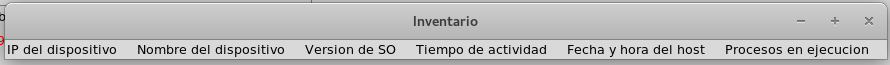
\includegraphics[width=.9 \textwidth]{images/inventario}
		\caption{Inventario.}
		\label{image:inventario}
\end{figure}
\FloatBarrier

En esta práctica se optó por recolectar las estadísticas vía SNMP de los siguientes recursos:

\begin{itemize}
	\item Porcentaje de memoria RAM en uso con OID 1.3.6.1.4.1.2021.4.6.0.
	\item Porcentaje de espacio en disco duro en uso (HDD) 1.3.6.1.2.1.25.2.3.1.6.1.
	\item Porcentaje de uso de CPU por núcleo 1.3.6.1.2.1.25.3.3.1.2.
\end{itemize}

Así mismo, es estableció un SLA en el que se indican 3 umbrales para los tres recursos seleccionados. A continuación podemos observar el uso en el programa desarrollado por el equipo en la figura \ref{image:umbrales}

\FloatBarrier
\begin{figure}[htbp!]
		\centering
			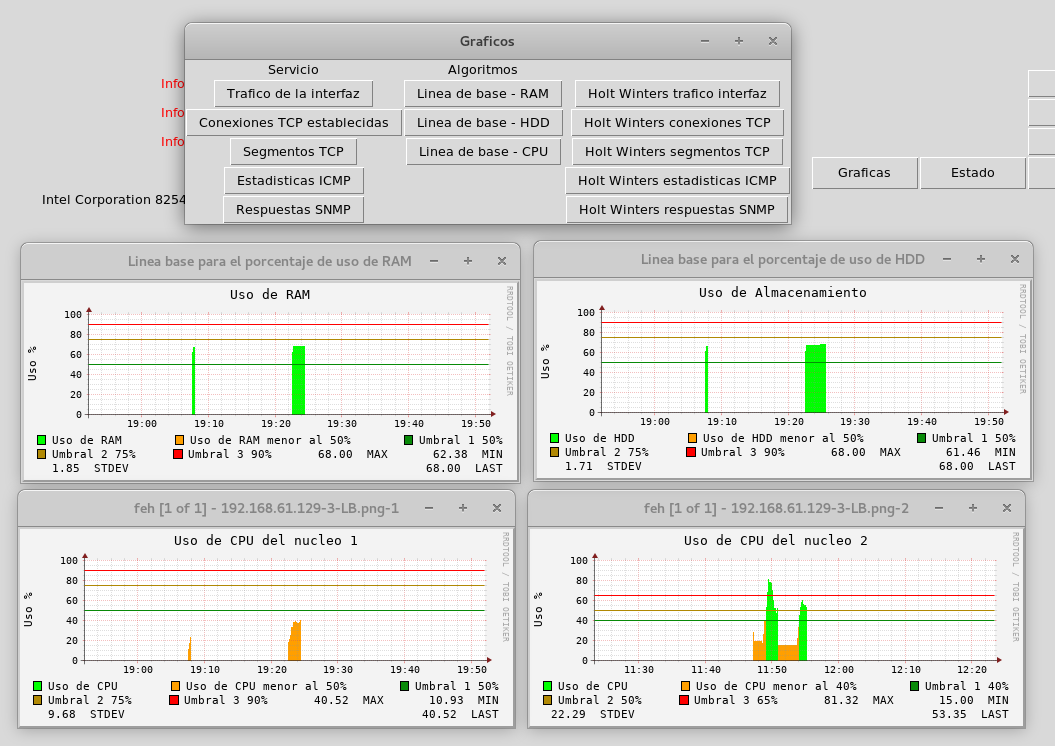
\includegraphics[width=.9 \textwidth]{images/umbrales}
		\caption{Umbrales de host.}
		\label{image:umbrales}
\end{figure}
\FloatBarrier

En la columna central de la ventana \textbf{Graficos} podemos observar tres botones: \textbf{Línea base - RAM}, \textbf{Línea base - HDD} y \textbf{Línea base - CPU}. Cada uno de ellos muestra la gráfica correspondiente.

Para el botón de \textbf{Línea base - RAM}, el programa despliega la gráfica situada debajo de la ventada de \textbf{Graficos} en el extremo superior izquierdo. Respectivamente, el botón de \textbf{Línea base - HDD}, el programa despliega la gráfica situada debajo de la ventada de \textbf{Graficos} en el extremo superior derecho. Por último, al presionar el botón de \textbf{Línea base - CPU}, el programa despliega una gráfica por cada uno de los núcleos de procesador con los que cuenta el agente. Estas gráficas son las que se encuentran en la parte inferior de la figura anterior.

Los umbrales establecidos fueron los siguientes:

\begin{itemize}
	\item 50\% como umbral Ready indicador de que el dispositivo puede necesitar atención en el futuro.
	\item 75\% como umbral Set indicador previo como alarma de inicio de una planeación para realizar reparaciones, actualizaciones o configuraciones nuevas.
	\item 90\% como umbral Go que indica falla o acción inmediata.
\end{itemize}

Dichos umbrales fueron establecidos con base en el comportamiento normal del agente. Es decir para los tres rubros (RAM, HDD y CPU) se utilizó como base un histórico del uso de recursos del hosts. De esta manera se definió el 50\% como umbral Ready ya que sólo en algunas ocasiones se alcanza este límite. Así mismo, el número de veces que se alcanza el umbral Set es menor e indica que es posible que el umbral Go sea alcanzado en un momento próximo. En este caso, podemos observar que tanto en RAM como en HDD el umbral Ready fue alcanzado pero sin llegar al umbral Set. En el caso del uso del CPU podemos observar que en el núcleo 1, ningún umbral fue alcanzado. Sin embargo, el núcleo 2 tuvo un pico fuera de lo normal que superó al umbral Set pero que no alcanzó al umbral GO.

Por último, se implementó un mecanismo de alarma vía correo electrónico que se activa cada que un host sobre pasa alguno de los umbrales. Este mecanismo es activado y ejecutado automáticamente por el programa. A continuación se muestra, los correos enviados:

\FloatBarrier
\begin{figure}[htbp!]
		\centering
			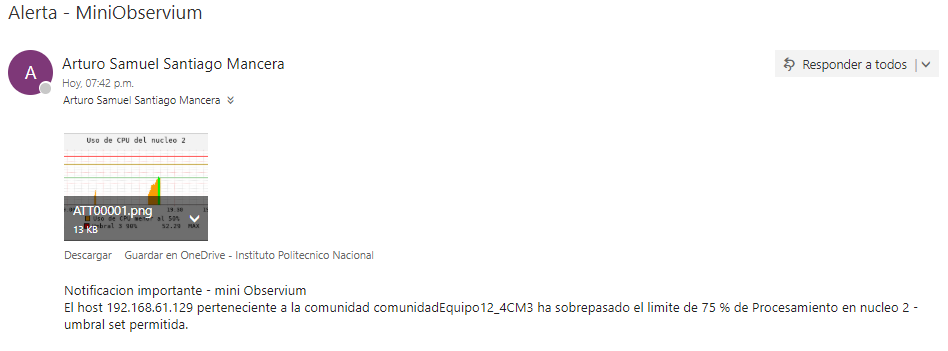
\includegraphics[width=.9 \textwidth]{images/correo1}
		\caption{Correo 1.}
		\label{image:correo1}
\end{figure}
\FloatBarrier

\FloatBarrier
\begin{figure}[htbp!]
		\centering
			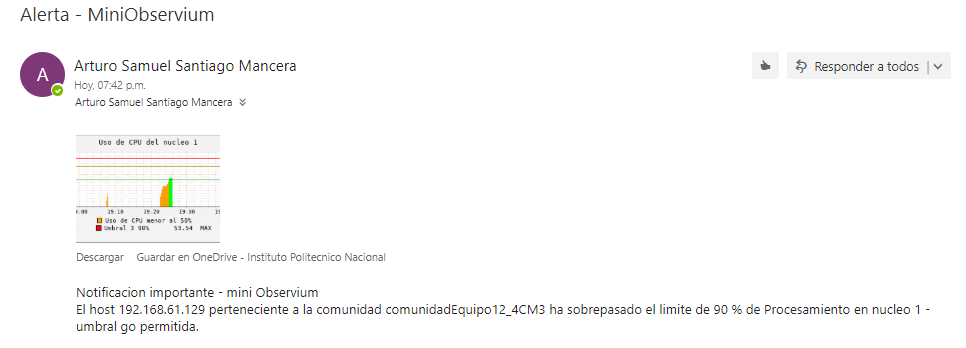
\includegraphics[width=.9 \textwidth]{images/correo2}
		\caption{Correo 2.}
		\label{image:correo2}
\end{figure}
\FloatBarrier

\FloatBarrier
\begin{figure}[htbp!]
		\centering
			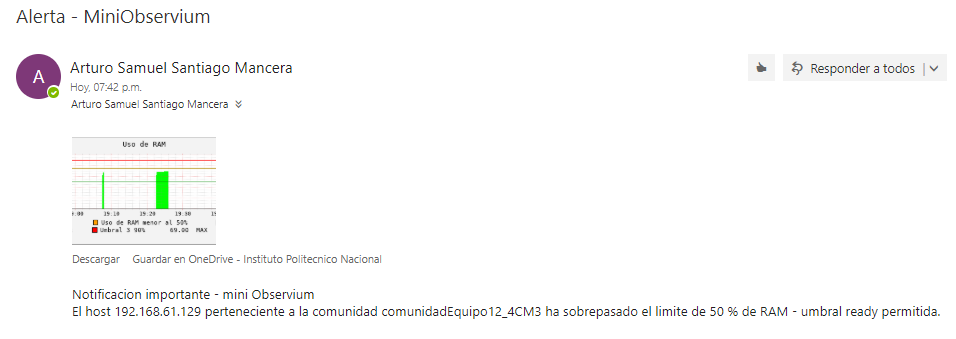
\includegraphics[width=.9 \textwidth]{images/correo3}
		\caption{Correo 3.}
		\label{image:correo3}
\end{figure}
\FloatBarrier